\documentclass{article}

\usepackage[utf8]{inputenc}
\usepackage[sorting=none]{biblatex}
\addbibresource{references.bib}

\usepackage{amsmath,amssymb,amsfonts}
\usepackage{hyperref}
\usepackage{graphicx}
\usepackage{textcomp}
\usepackage{caption}
\captionsetup[figure]{font=small}
\usepackage{xcolor}
\usepackage{geometry}
\geometry{
    top=3cm,
    bottom=3cm,
 }

\usepackage{subfigure}
\usepackage{float}

\usepackage{setspace}
\usepackage{lipsum}

\usepackage{multicol}
\setlength{\columnsep}{1cm}

\begin{document}

\begin{titlepage}
\newgeometry{top=2cm,bottom=2cm}

\hspace*{-0.5cm}
\includegraphics[width=2.5cm]{um-logo.png} \\

\vspace{2cm}

\begin{center}
    
    \vspace{2cm}

    {\huge
    \begin{spacing}{1.0}
        \textbf{(Re-)Discovering Forbidden Minors For Treewidth}
    \end{spacing}
    }
        

    \vspace{0.5cm}                                                                              
    {\LARGE
    \begin{spacing}{1.0}
     Finding 90-100 'folklore-only' minimal forbidden minors in F(4) and an initial list in F(5)
    \end{spacing}
    }

    \vspace{2cm}
        
    {\LARGE \renewcommand{\arraystretch}{1.2}
        \begin{tabular}{c}
            Diogo Rio \\
        \end{tabular}
    }
    
\end{center} 


\vfill
\begin{flushleft}
    { \large
    \textbf{Data Science and Artificial Intelligence} \\  
    BSc. Thesis @ Maastricht University \\  
    Fall \& Spring 2023 (18 ECTS) \\ 
    \textbf{Supervisor \& Examiner:} Steven Kelk \\
    \textbf{Co-Supervisor:} Ruben Meuwese \\
    \textbf{Examiner:} Matúš Mihalák \\
    }
\end{flushleft}

\restoregeometry
\end{titlepage}
\begin{multicols}{2}
\date{}
\section*{Abstract}
The aim of this thesis is to explore the efficiency of algorithms dedicated to finding minimal forbidden minors in $F(4)$, where $F(k)$ is the finite set of graphs with the following property: a graph $G$ has treewidth at most $k$ if and only if none of the graphs in $F(k)$ are a minor of $G$. The treewidth of a graph is a fundamental characteristic that describes its resemblance to a tree. This is crucial in graph theory, as it enables polynomial time solutions for NP-hard problems, for graphs with bounded treewidth. Methods of communicating the discovered forbidden minors to the community in a verifiable manner are developed, as only up the set $F(3)$ are they fully known. Finally, the research aims to analyze the exhaustiveness of the obtained list of forbidden minors in $F(4)$, as well as examine the feasibility of extending the algorithms used in $F(4)$ in generating a non-exhaustive list for $F(5)$.\par To achieve these goals, the study employs graph generation and exploration techniques, search-space pruning methods, and connectivity and isomorphism checks. Different approaches are evaluated, and a MySQL database structure is implemented to facilitate the sharing of any research outcomes.\par It defines an endeavor to advance the field of algorithmic graph theory and its possible applications in solving complex computational problems.\par
\vspace{0.5cm}
% Keywords (may be sorted in alphabetical order)
\noindent
\textbf{Keywords:}
Forbidden Minors, Treewidth, NP-hardness, Pruning, Connectivity, Isomorphism
\section*{Acknowledgment}
I would like to use this section to thank my supervisor Steven Kelk, for the guidance throughout the project - as well as for suggesting the topic.
\renewcommand*
\contentsname{Table of Contents}
\tableofcontents

\section{Introduction}

\subsection{Contextualization}
Folklore, unproven theories, talk about the existence of around 90 to 100 minimal forbidden minors in F(4). This is, however, unknown, and simply intuition-based by some researchers of the topic.

What is known is that a finite limit does exist. As a starting point, the sets F(1), F(2), and F(3) are known and fully proven to be fully enumerated. Nothing of the sort composes the case for k $>$ 3.

Therefore, the foundation of this thesis is held.

The importance of this task has to do with the fact that analyzing the treewidth of a graph may allow us to make fair conclusions regarding the computational time of NP-hard problems.

\subsection{Thesis Outline}
This thesis looks to explore the nature of the algorithms that allow the generation of graphs as well as discern relevant pruning techniques that may significantly reduce the time spent searching the space.

Different tools are used, not always in the same environment/language, so to speed up the entire process of filling F(4) and F(5). For this reason, conversions are regularly conducted to allow compatibility between functions and their results.

A MySQL database structure is also implemented to provide the possibility of sharing the results obtained by this research. 

All these algorithms, methods of conversion and sharing are thus described throughout the paper.

\subsection{Problem Statement }
[Look into what it could be]
\subsubsection{Research Questions}
Here are some of the questions the research aims to address:

1. How can we algorithmically efficiently discover the list of 90 to 100 minors for F(4)?

2. How can the list of minors we find be communicated to the community, in a verifiable way?

3. Is there any evidence that this list for F(4) is (or is not) exhaustive?

4. Can the same algorithmic techniques be used to produce a (non-exhaustive) list for F(5)?


\section{Methods}
The methods used within the thesis are of various natures. Some focus on generating or collecting a valid database, others on analyzing them. There were efforts to efficiently and sequentially fill the database with correct findings, as the algorithms ran throughout the semester. In this section, one can take a deeper look into what comprises the system of the project.

\subsection{Graph Generation}
Regardless of the chosen approach, a shared necessity was generating a valid set of graphs that would be fed into the algorithms that discern critical forbidden minors. With that in mind, it became a fair starting point to understand the basic fundamentals of the types of graphs that were to be found. In other words, at the most basic of levels, all (minimal) forbidden minors naturally have a few structural characteristics in common. At the very least, they are always connected, with no vertices without any edge connecting them to the rest of the graph. They are also undirected, which means the sense of direction is irrelevant and therefore unnecessary to model, as are edge weights.

Another important characteristic to monitor is graph isomorphism. There was a need to find a way to guarantee that any minor that was identified could not be rearranged into one same one that had been found previously. There are two ways of doing this: either through a post-analysis concept called isomorphism-checking or by modeling unlabelled graphs from the beginning, which revolves around the idea of not giving a particular ID (or label) to each of the graph vertices. The latter would inherently be a method of isomorphism checking but would limit the amount of graph generation tools that could be used. For that reason, and given the fact that applying restrictions from the conception of the thesis would most likely hinder its development, the option chosen was the former. There is already a significant number of efficient isomorphism-checking tools, which translates into more time focused on the task at hand.

\subsubsection{Combinatorial (Exhaustive) Graph Enumeration}
The combinatorial graph enumeration graph generation approach is a naive one. It consists in exhaustively conceiving all graphs with any provided number of vertices. This approach is designed manually and can therefore be logically built with the fundamental graph characteristics mentioned previously. This means the outcomes of this method would result in having every valid graph, ready for analysis. Exhaustively generating graphs sounds promising - if it weren't for the fact that the number of possible combinations increases exponentially \cite{oeisA001349}. Brute-forcing through the number of vertices is therefore not computationally feasible in the long term.

Nevertheless, the fact that it guarantees exhaustiveness is quite tempting. There is the certainty that no graphs are overlooked. For that reason, this approach is kept up to a reasonable number of vertices, established to be 7, where it significantly outperforms random graph sampling. That is easily explainable, as the number of possible combinations of vertices and edges is small enough to justify the safety of exhaustiveness. With random sampling, the loom of having at least a graph missing is always present.

The combinatorial graph enumeration algorithm was based on Arseny Khakhalin's work \cite{khakhalin2020}. It generates graphs recursively, by including or skipping each edge, using a lexicographical order of construction. Again, it performs well up to 7 vertices. Venturing over that number, however, starts to become seriously challenging, since the computational time increases by $2^{n-1}$ with each vertex increase. An alternative approach was thus worth considering.

\subsubsection{The Package 'nauty': Possibilities and Limitations}
The package 'nauty' is an old library developed in and for C. It is a set of procedures that aims to, among many other functionalities, quickly compute several graph operations, such as isomorphism and canonical labeling. A very useful program for this thesis would have been 'geng', included within 'nauty'. This program gives the user the ability to efficiently (and exhaustively!) enumerate non-isomorphic graphs. By tweaking certain parameters, it was possible to have it generate the types of valid graphs desired - connected and specific to the number of wanted vertices.

Once again, this presented itself as a promising approach (and as it will be suggested later on, it may very well still be). However, a setback surged. The format with which 'nauty' outputs its results is an unusual one, developed with the intent of reducing the size of the files containing them. It is a smart procedure since by using the .g6 file format, any usual graph representations (edge lists, adjacency matrices or lists, ...) can be diminished tremendously, while the program itself remains able to interpret any of those entries. Unfortunately, this distinguished factor limited making consistent use of 'nauty'. The conversion attempts (from .g6 files to ones containing any usable graph representations) were in vain. The Python functions I tried applying were prone to incorrect conversions, and this was the main reason why this approach was dropped and yet another alternative was considered.

\subsubsection{Random Binomial Graph Sampling}
Random sampling: a good solution to many computational intractability roadbloacks. After the somewhat inconsequential previous two methods, random sampling seemed like an interesting change of pace. Until it became an unrealistic effort (i.e. until the sample became measly in comparison with the possibly generatable graphs), it could yield a significant number of results for a number of vertices higher than 7. This was worth following, as it can undoubtedly generate some more valid graphs, which is progress towards finding more forbidden minors after all.

The random graph sampling approach used was based on the Erdős–Rényi model. Essentially, the method generates a set of graphs based on but a few parameters: the number of vertices in the graph to be created, the probability of any two vertices being connected by an edge (i.e., whether an edge is created, independently randomly sampled between every pair of vertices), and lastly the actual number of samples to be generated with these conditions.

Sequentially, this model also filters out any graphs that are not connected, pruning the search space from irrelevant graphs. The isomorphism check could be conducted at this stage, however, given the program was developed to run many times, each time trying to find new elements of $F(k)$, it is more efficient to only perform the isomorphism check on all the graphs that survive the conditions that will be explained in the following sections. That is because iterating through such a possibly large sample, in what is arguably the most time-consuming task of the final program, is not beneficial. The isomorphism checking always needs to be done anyway when graphs are on the verge of being added to the database - so that there is a certainty that any added graphs are indeed \textit{new} minimal forbidden minors.

\subsubsection{The Combined Approach}
In the end, the graph generation approach which was chosen to be the main one was a junction of both the ones developed.

As suggested earlier, the feasibility of guaranteeing exhaustiveness up to 7 vertices is something worth chasing. For that reason, the combined approach was settled using combinatorial graph enumeration up to that threshold, and random sampling thereon.

\subsection{Forbidden Minor Finding}
After there is a set of graphs to work with, it is necessary to perform the actual analysis of it. Minimal forbidden minors are thus identified through a method that logically applies the conditions of what it means 'to be minimal'.

\subsubsection{Simplifying the Forbidden Minor Finding through Conditioning}
Without having to dive too profoundly into the theory of forbidden minors, it is possible to discern how a sub-graph can be minimal. Since the forbidden minors at focus in this thesis are related to the treewidth of a graph, the observable change in the treewidth itself, as we apply vertex/edge deletion and edge contraction, is sufficient to determine the \textit{minimality} of a minor.

All in all, what the method does is apply the three basic conditions of what it means to be a graph minor - all while constantly checking for any treewidth alterations that may originate from it. Recalling, a minor is the resulting sub-graph $G$ obtainable from an original graph $H$ by subjecting $H$ to operations such as deleting a vertex, deleting an edge, or contracting an edge, for each instance of a vertex or an edge. If the treewidth upon doing so does \textit{not} decrease, then one can be sure that \textit{minimality} is yet to be achieved.

In practical terms, what all this theory means is the following: 

For each generated graph $G$, $tw(G)$ is initially checked. If its treewidth is different from the established treewidth reference (which is always $k+1$), $G$ is discarded. Discarding a graph means that the graph cannot possibly be a minimal forbidden minor. These three upcoming steps can be done in arbitrary order. Next, for each vertex in the graph, that vertex is removed. $tw(G)$ is checked again. If there exists a vertex $v$ such that deleting $v$ does not cause the treewidth to decrease, the graph is dropped. The same exact process is also done for each edge in the graph, where that edge is removed. Finally, the same process is yet again conducted for each edge in the graph, this time contracting it. Surviving all these conditions represents the finding of a minimal forbidden minor. Whether a new one or not, that is to be determined at a later stage. 

Any discarded graphs are abandoned and not further looked into, as not doing so (i.e. not abandoning them) would heavily impact the run-time and limit the sample size that could realistically be analyzed. Long term, it is heavily inefficient to perform analysis as we deconstruct a graph, as the samples are not representative of all the graphs that exist. The experiment conducted on this further corroborates this decision (see 3.4).

Regardless, a necessary aspect for this method to work is, naturally, having an exact (and not purely heuristic) treewidth solver.

\subsubsection{\textit{QuickBB}: The Exact Treewidth Solver}
With the goal of knowing the true treewidth of a graph in mind, the program has the $QuickBB$ algorithm \cite{gogate2004} incorporated within it. It is a Branch and Bound optimization algorithm that computes the treewidth of any given undirected graph. It works by performing a search in the perfect elimination ordering of graph vertices space, using theory-based pruning and propagation techniques. An important characteristic that is behind the choice of this algorithm is the fact that it improves upon alternative methods, such as $QuickTree$, which is a complete algorithm \cite{gogate2004}. 

Advantages such as its good anytime performance, resulting in unprecedentedly accurate upper bounding on graphs whose optimal treewidth had not been feasible until the development of $QuickBB$, contributed heavily towards adopting (and adapting) this method. Nowadays, however, it is true that $QuickBB$ is outperformed by alternative C++ or Java solvers, such as $BestTW$ or $BFHT$ \cite{dow2007}. The reason behind using $QuickBB$ despite the known outperformers is that newer solvers are not readily available in Python, which was the language used in this thesis. Besides, the computed treewidths in this project were small, after all - which removes the need for current state-of-the-art solvers.

\subsubsection{Isomorphism Checking}
Another important aspect of assuring the preciseness and validity of the database is isomorphism checking. Formally, two graphs $G$ and $H$ are isomorphic if there exists a bijection between their vertex sets in a way that for any pair of vertices $v_1$ and $v_2$ in $G$, there exists a corresponding pair of vertices $u_1$ and $u_2$ in $H$ (and vice-versa), such that the presence or absence of edges is preserved. Essentially, shared graph morphologies, with different labels. Having hidden repeated entries is an endangering issue, as it would contribute towards getting the wrong feel and number of results. 

Therefore, firstly, the program - upon being on the verge of adding a minimal forbidden minor into the database - collects all the already existing instances from the specific table it is meant to add into. This collected set then refers to the set of identified forbidden minors in the current program run and performs a one-on-one comparison between every element of both sets, using the $vf2$ algorithm, which performs well on large graphs \cite{foggia2001}. This is thus the final condition separating a found forbidden minor from being added into the database. If it does happen to be a newfound minimal forbidden minor, structurally different from all its peers, it progresses onto the database, finishing the entire forbidden minor finding process.

\subsection{The Idea of Designing a Database}
The designed program is not single-run. What this means is that in order to find a reasonable number of forbidden minors, the program is intended to run multiple times, because otherwise, it would be computationally impossible to achieve results. In answer to this, a database proved to be an interesting approach, since it can be updated and published externally through various means. Any issues that the program faces are independent of the database, keeping it a safe method to store any outcomes. This is called data persistence, which is a vital advantage in computationally intensive programs such as this one.

The fact that instances can be easily distinguishable from one another, by categorizing graphs with additional parameters also helps with the handling of the data. The versatility and scalability advantages that come with a database are of such importance that in truth an alternative option was never seriously considered.

Yet, this is not all. The familiarity with MySQL and the uncertainties at the beginning of how the findings would be communicated in the end were equally major influences.

\section{Experiments}
<empty>

\subsection{e.g.}
<empty>

\subsubsection{e.g}
<empty>
\section{Results}
<empty>

\subsection{e.g.}
<empty>

\subsubsection{e.g}
<empty>
\section{Discussion}
<empty>
\section{Conclusion}

The program was capable of re-discovering the minimal forbidden minors for $F(1)$, $F(2)$, $F(3)$, as well as identifying a number of elements of $F(4)$ and $F(5)$. All the generated minimal forbidden minors are publicly available online, and can be subject to verification through a panoply of means, given the panoply of formats published. On the procedure itself, the obvious limitation of the approach were algorithmic. There is a formidable number potential candidate graphs and it is challenging to efficiently enumerate or sample in such large spaces. Nevertheless, it is possible to identify a number of areas that can be dived upon for improvement in future research. On one hand, it would be useful to tune the graph generation procedure, so that graphs that cannot possibly be minimal forbidden minors (e.g. graphs with nodes of degree 2, graphs with multiple biconnected components, etc.) are never generated. Essentially, more extensive and focused pruning mechanisms. Relatedly, one could explore sampling via the topic of k-trees, which are edge-maximal graphs for a given treewidth. Above all, more ambitious algorithm engineering is bound to achieve the goal of finding close to 90 to 100 forbidden minors in $F(4)$, and likely for higher values of $k$ too. It would help if the constituent parts of the pipeline were to run more quickly, or simply more efficiently. A collaborative approach, which looks to farm out graphs (in the style of SETI@Home \cite{seti2002}) out of a fully enumerated online database would be an interesting way forward. Perhaps using the 'nauty' swift and light C++ generation tool 'geng' (using the .g6 file format), converting those graphs into a format this program can work with and constantly updating the results is one way of guaranteeing exhaustiveness. The hosting of such a service would then be available for any researchers willing to spend CPU resources on the search for minimal forbidden minors. Going forward, a public ever-evolving forbidden minor database and online checking tool would be an exciting outcome of the concepts tackled in this thesis.
\newpage
\printbibliography 
\newpage
\section*{Appendix}

Additional minimal forbidden minors for $F(4)$: \par
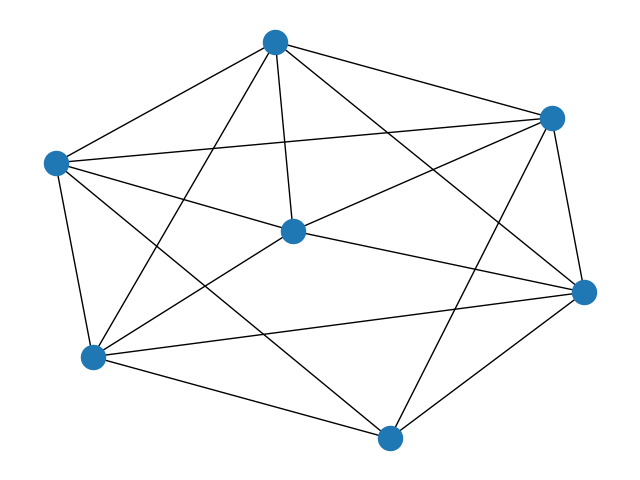
\includegraphics[width=3.25cm]{images/mfms/f4_2.png}
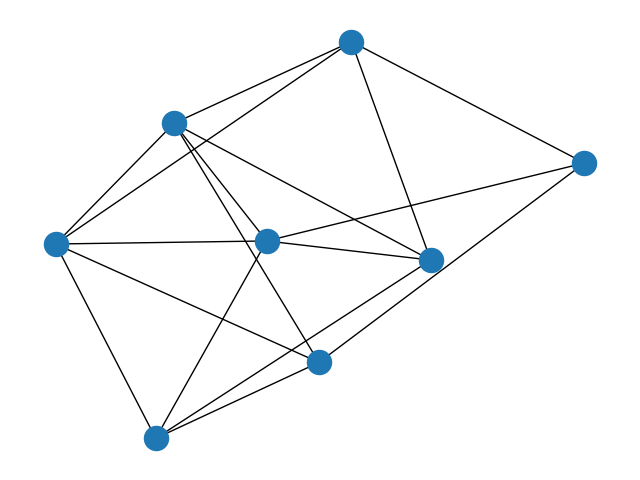
\includegraphics[width=3.25cm]{images/mfms/f4_4.png}
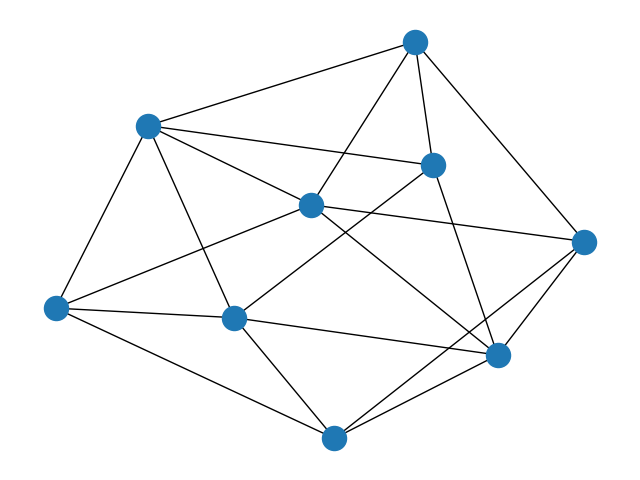
\includegraphics[width=3.25cm]{images/mfms/f4_6.png}
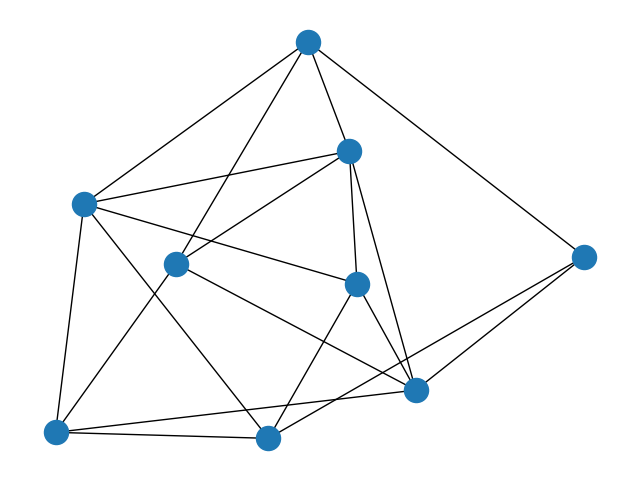
\includegraphics[width=3.25cm]{images/mfms/f4_7.png}
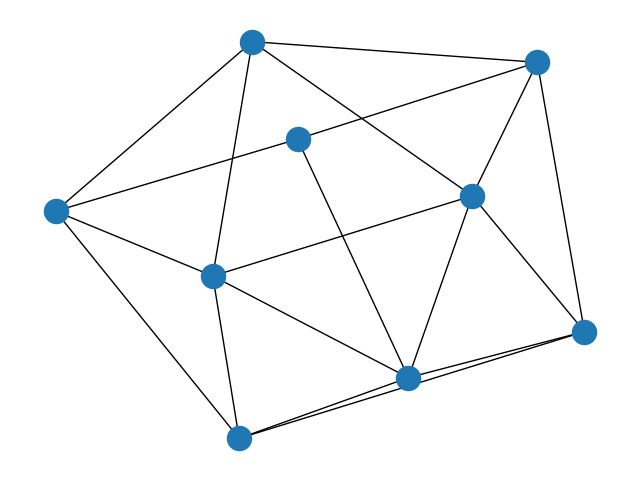
\includegraphics[width=3.25cm]{images/mfms/f4_8.png}
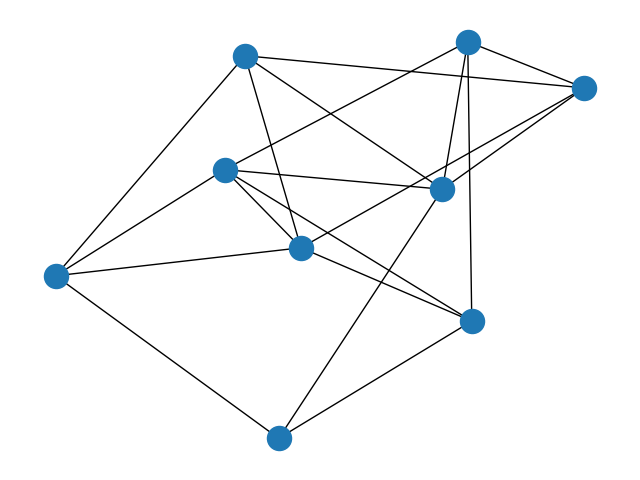
\includegraphics[width=3.25cm]{images/mfms/f4_10.png}
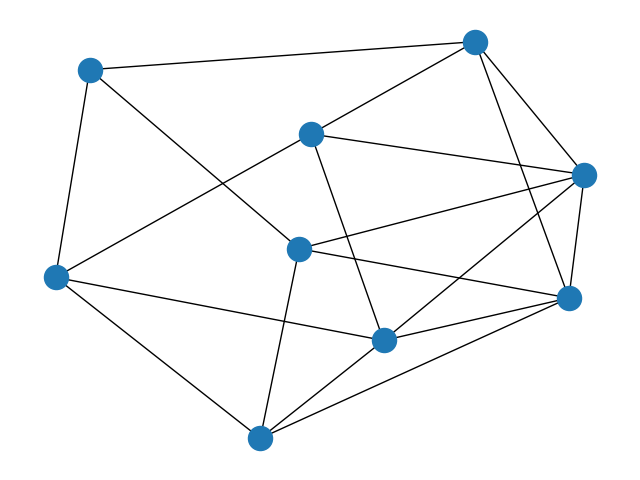
\includegraphics[width=3.25cm]{images/mfms/f4_11.png}
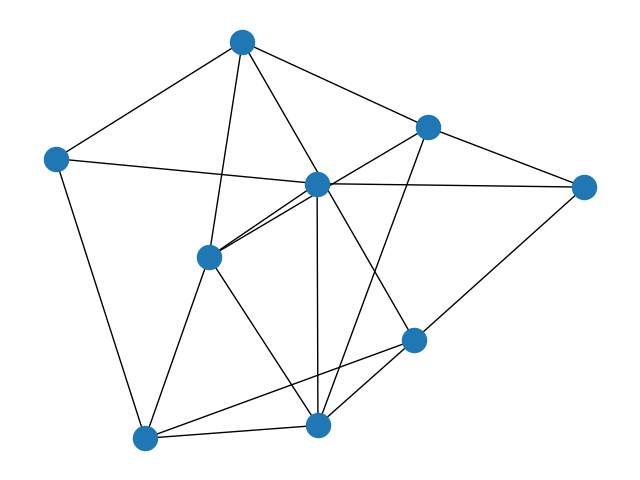
\includegraphics[width=3.25cm]{images/mfms/f4_12.png}
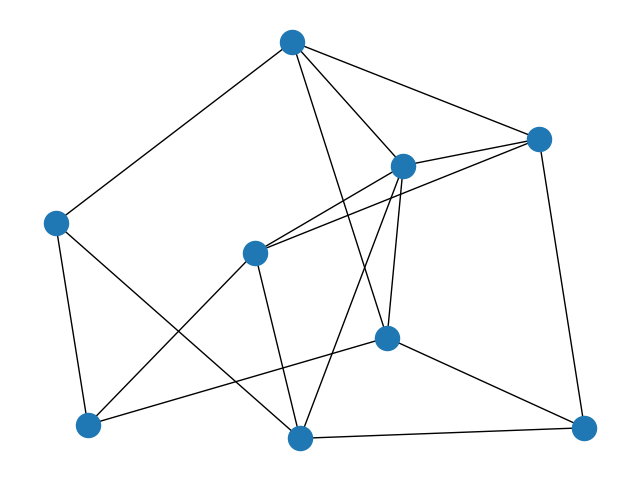
\includegraphics[width=3.25cm]{images/mfms/f4_13.png}
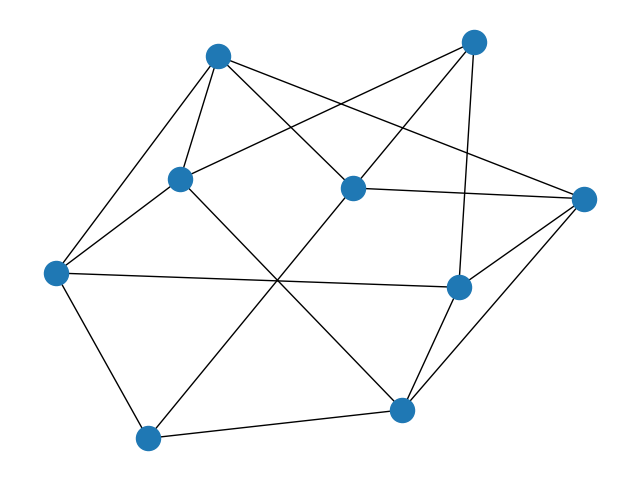
\includegraphics[width=3.25cm]{images/mfms/f4_14.png}
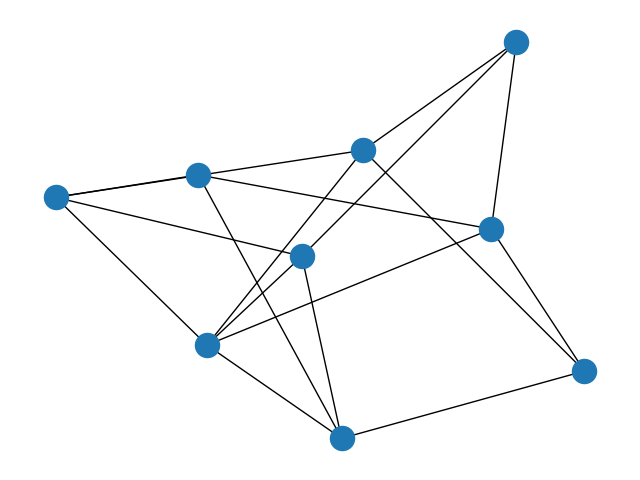
\includegraphics[width=3.25cm]{images/mfms/f4_15.png}
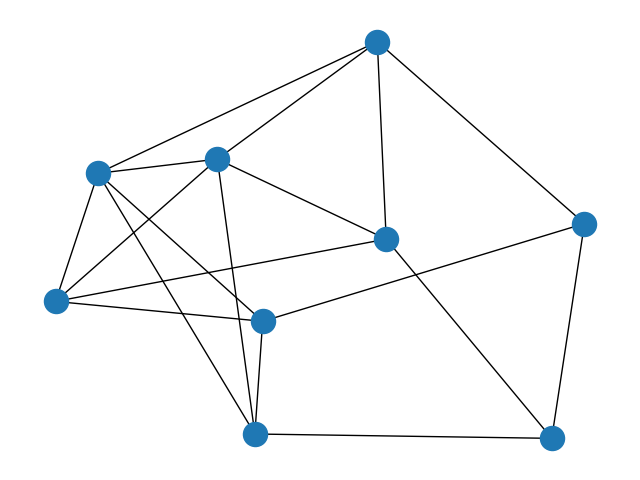
\includegraphics[width=3.25cm]{images/mfms/f4_16.png}
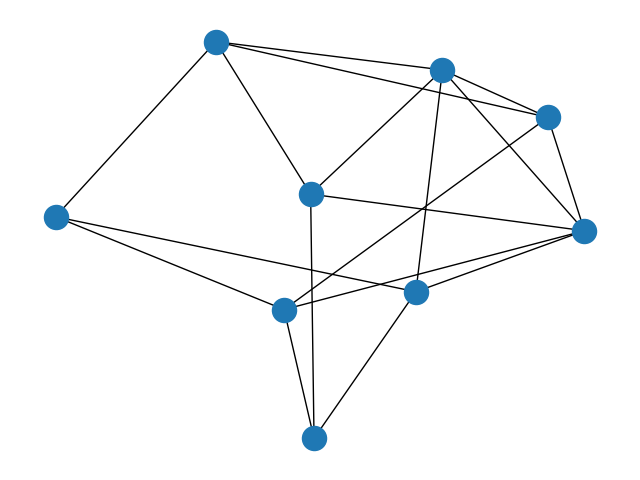
\includegraphics[width=3.25cm]{images/mfms/f4_17.png}
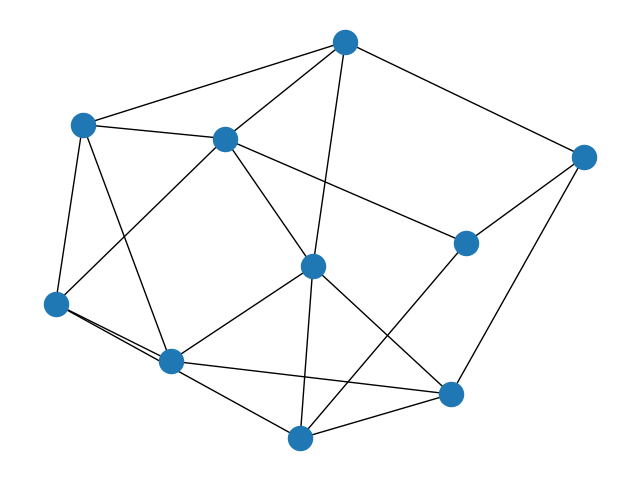
\includegraphics[width=3.25cm]{images/mfms/f4_18.png}
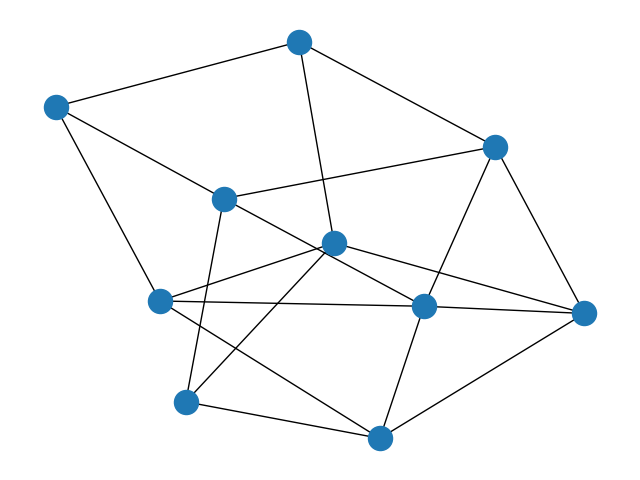
\includegraphics[width=3.25cm]{images/mfms/f4_19.png}
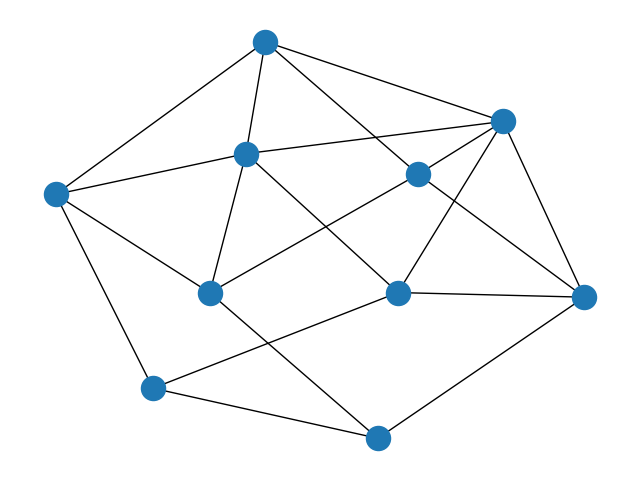
\includegraphics[width=3.25cm]{images/mfms/f4_20.png}
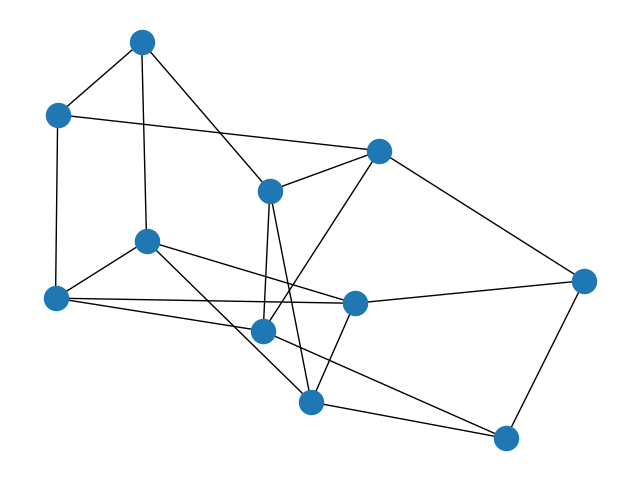
\includegraphics[width=3.25cm]{images/mfms/f4_21.png}
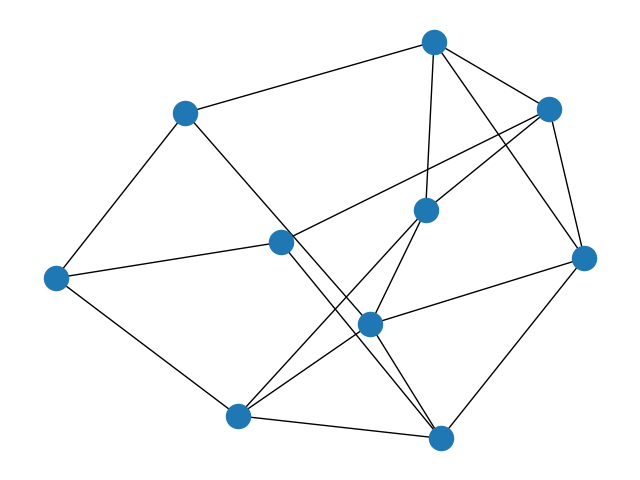
\includegraphics[width=3.25cm]{images/mfms/f4_22.png}
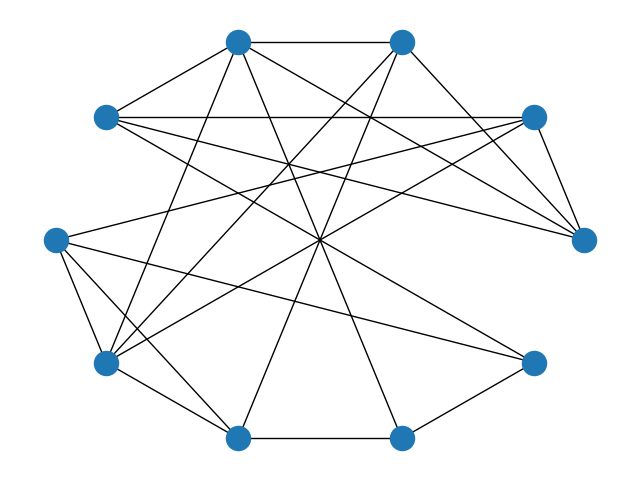
\includegraphics[width=3.25cm]{images/mfms/f4_23.png}
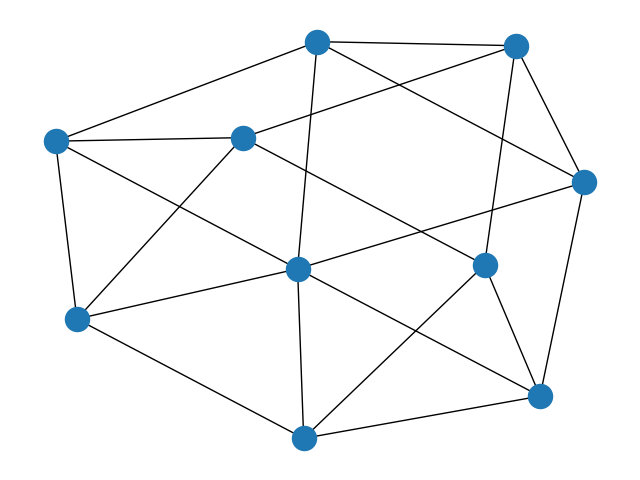
\includegraphics[width=3.25cm]{images/mfms/f4_24.png}
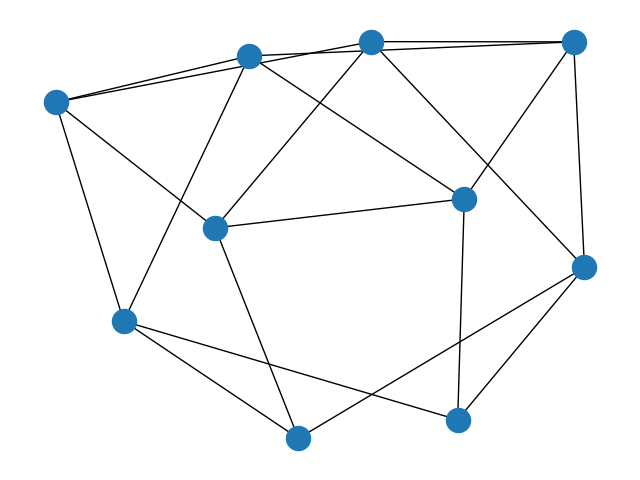
\includegraphics[width=3.25cm]{images/mfms/f4_25.png}
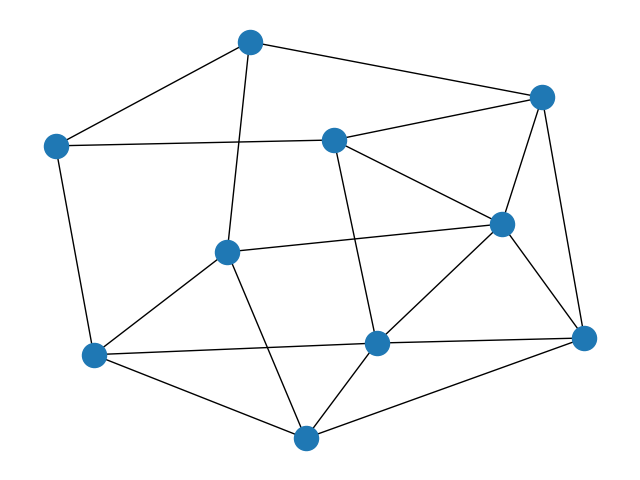
\includegraphics[width=3.25cm]{images/mfms/f4_26.png}
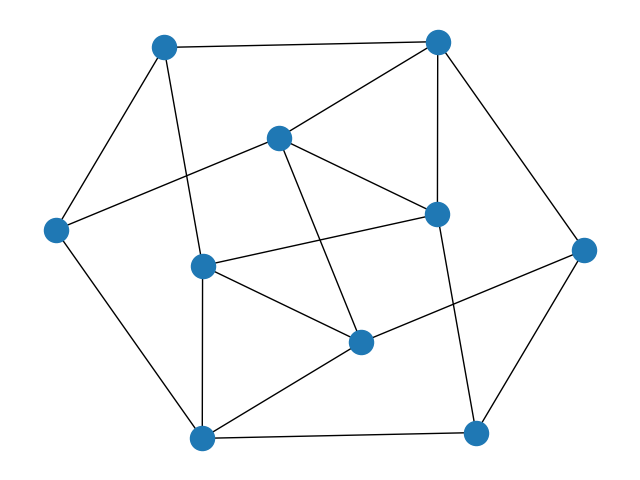
\includegraphics[width=3.25cm]{images/mfms/f4_27.png}
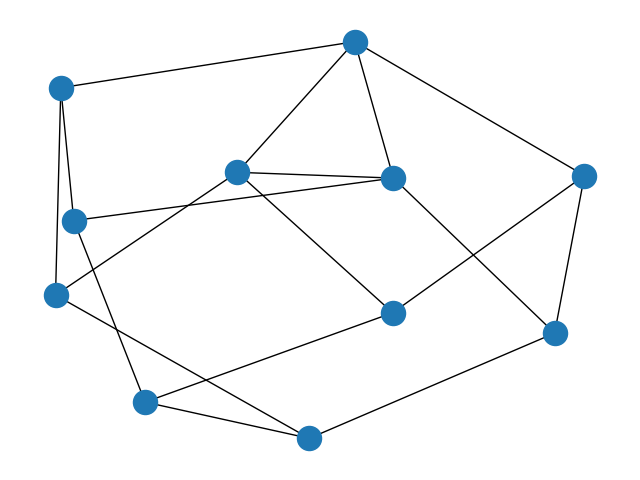
\includegraphics[width=3.25cm]{images/mfms/f4_28.png}
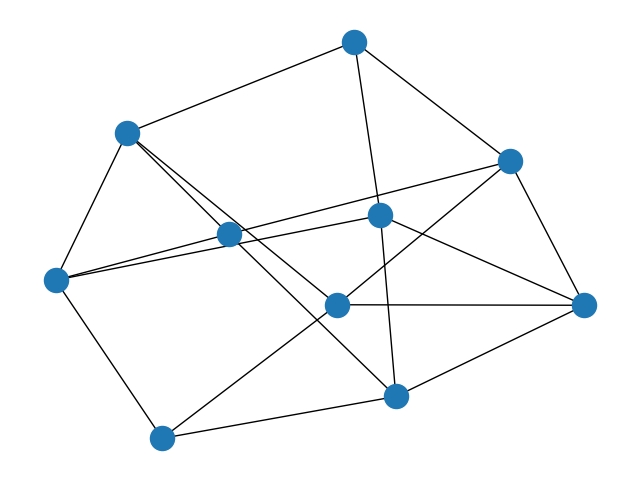
\includegraphics[width=3.25cm]{images/mfms/f4_29.png}
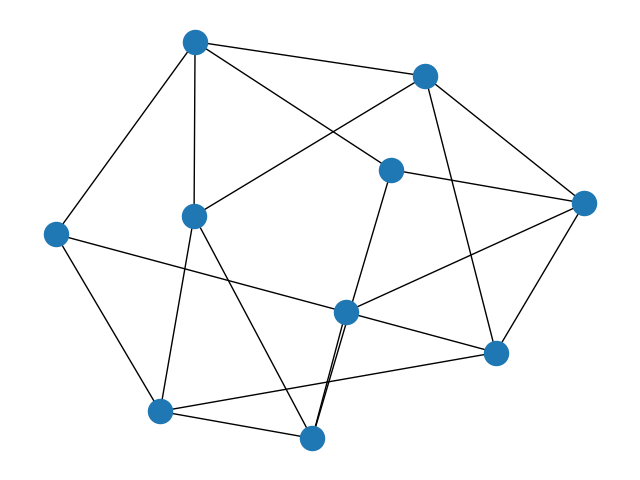
\includegraphics[width=3.25cm]{images/mfms/f4_30.png}
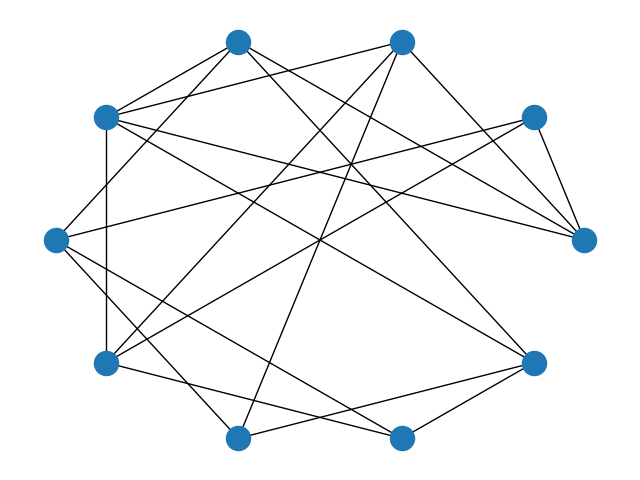
\includegraphics[width=3.25cm]{images/mfms/f4_31.png}
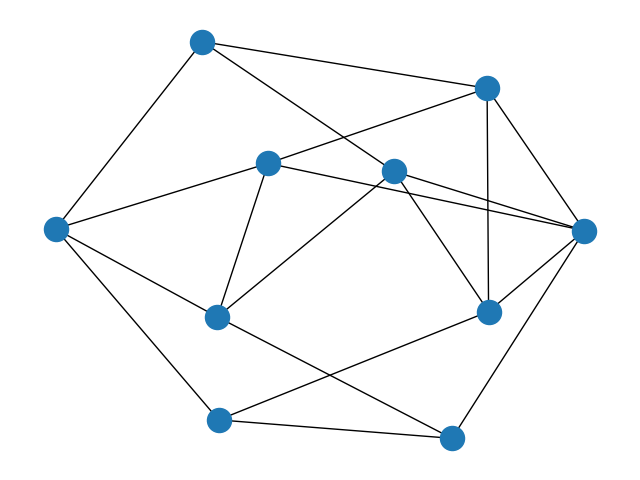
\includegraphics[width=3.25cm]{images/mfms/f4_32.png}
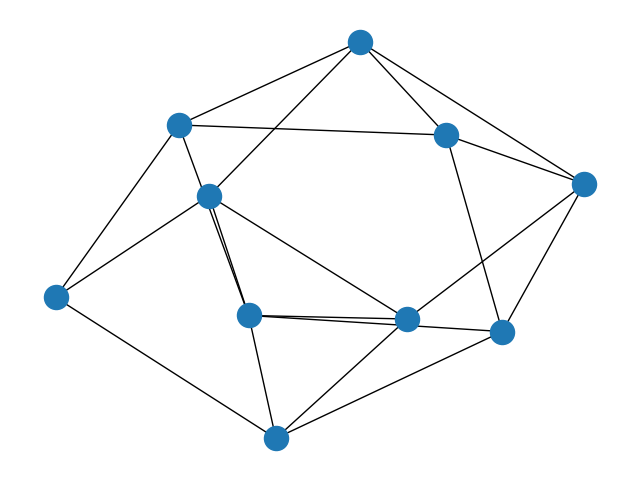
\includegraphics[width=3.25cm]{images/mfms/f4_33.png}
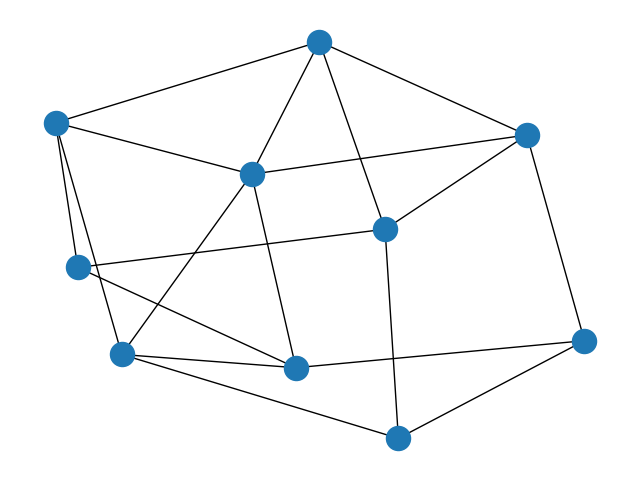
\includegraphics[width=3.25cm]{images/mfms/f4_34.png}
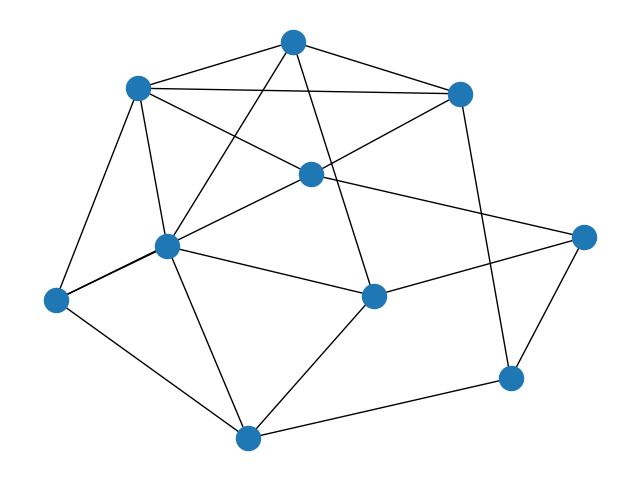
\includegraphics[width=3.25cm]{images/mfms/f4_35.png}
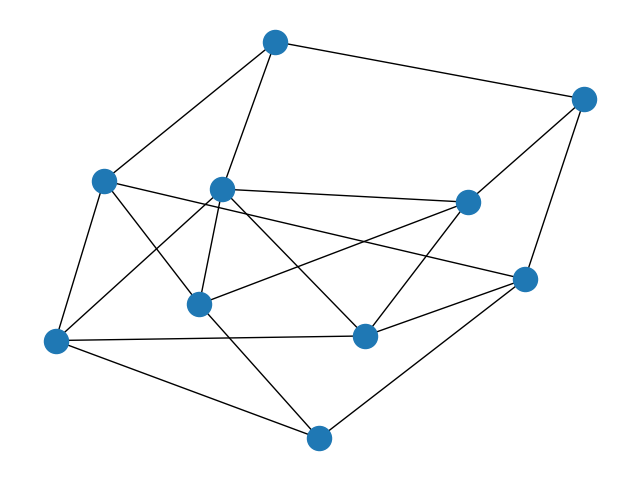
\includegraphics[width=3.25cm]{images/mfms/f4_36.png}
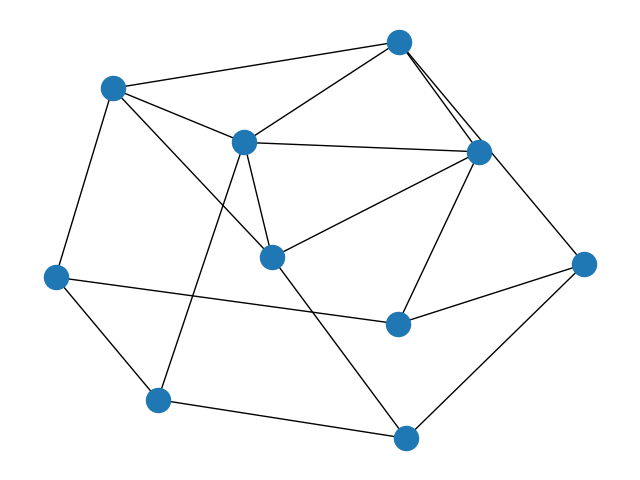
\includegraphics[width=3.25cm]{images/mfms/f4_37.png}
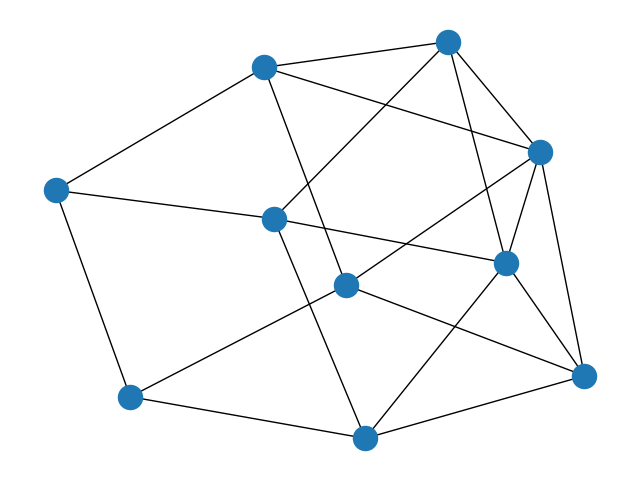
\includegraphics[width=3.25cm]{images/mfms/f4_38.png}
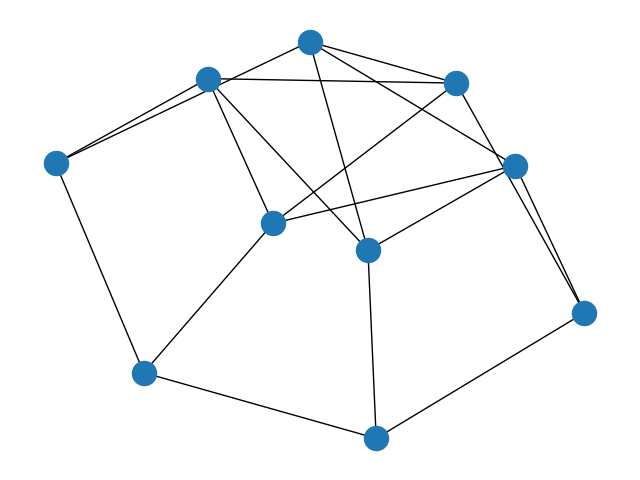
\includegraphics[width=3.25cm]{images/mfms/f4_39.png}
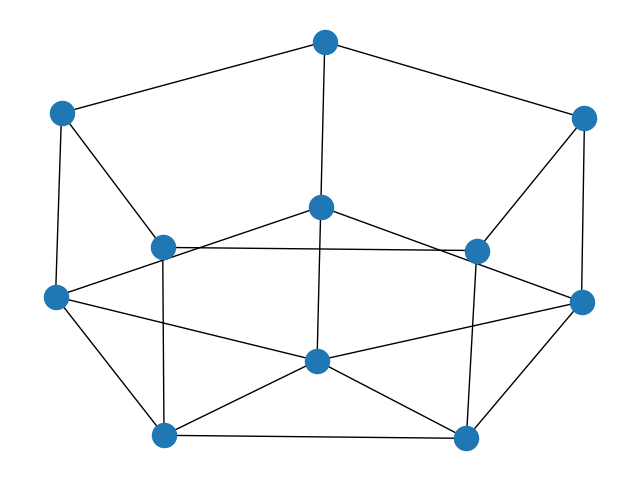
\includegraphics[width=3.25cm]{images/mfms/f4_40.png}
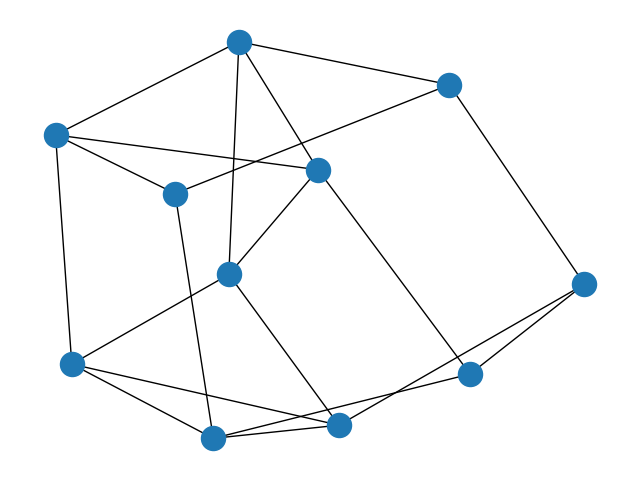
\includegraphics[width=3.25cm]{images/mfms/f4_41.png}

\newpage
Additional minimal forbidden minors for $F(5)$: \par
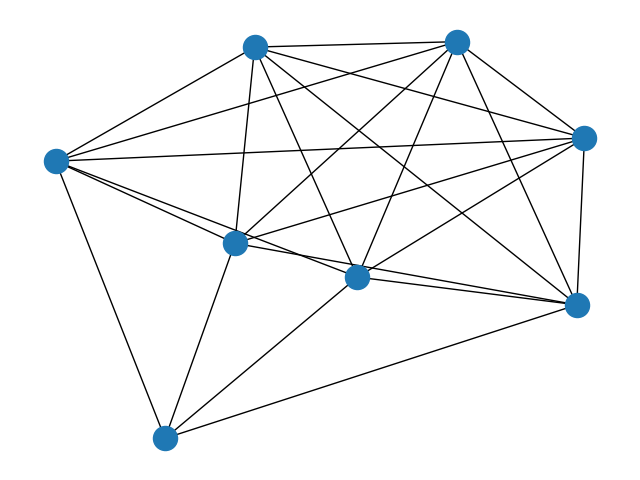
\includegraphics[width=3.25cm]{images/mfms/f5_3.png}
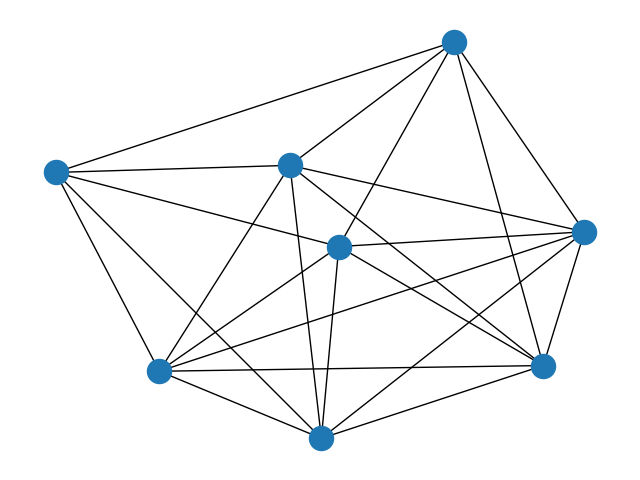
\includegraphics[width=3.25cm]{images/mfms/f5_4.png}

\end{multicols}

\end{document}